%%%%%%%%%%%%%%%%%%%%%%%%%%%%%%%%%%%%%%%%%%%%%%%%%%%%%%%%%%%%%%%%%%%%%%%%%%%
%% ws-procs9x6.tex   :   20-9-2004
%% Text file for Proceedings Trim Size [9in x 6in] written in Latex2E.
%% The content, structure, format and layout of this style file is the 
%% property of World Scientific Publishing Co. Pte. Ltd. 
%% Copyright 1995, 2002 by World Scientific Publishing Co. 
%% All rights are reserved.
%%
%% Proceedings Trim Size: 9in x 6in
%% Text Area: 7.35in (include runningheads) x 4.5in
%% Main Text is 10/13pt					  
%%%%%%%%%%%%%%%%%%%%%%%%%%%%%%%%%%%%%%%%%%%%%%%%%%%%%%%%%%%%%%%%%%%%%%%%%%%

%% Use \tbl{...} command for table caption i.e. to fit table width.
%% Use \caption{...} command for figure caption.
%\documentclass[draft]{ws-procs9x6}  
\documentclass{ws-procs9x6}
\usepackage{pgf}
\usepackage{tikz}


%\pgfdeclareimage[width=2cm]{nefroideIdeal}{nefroideIdeal}



\begin{document}

\title{Level Sets}

\author{Raquel Pezoa}

\address{Universidad T\'ecnica Federico Santa Mar\'ia, \\
Avenida Espa\~na 1680, \\ 
Valpara\'iso, Chile\\ 
E-mail: rpezoa@usm.cl}

%\author{T.~R. SIMON, S. CLARKE and S.~N. GERALD}

%\address{World Scientific Publishing Co Ltd, \\ 
%57 Shelton Street, \\
%London WC2H 9HE, England\\
%E-mail: wspc@wspc.ox.uk}  

\maketitle

\abstracts{
Ac\'{a} debe ir el abstract.}

\section{Curve Evolution}
%Lecture Notes in Mathematics
%Editors:
%J.–M. Morel, Cachan
%F. Takens, Groningen
%B. Teissier, Paris


The numerical analisys of the motions of plane curves driven  by a function of
the curvature. If $C$ is a smooth (say $C^{2}$) curve, they are described by a
partial differential equation (PDE) of the type:

$$\frac{\partial C}{\partial t}=G(\kappa)\bold{N}$$

$$\kappa= \text{ curvature}, \ \ \ \bold{N}=\text{ normal vector to the curve}$$

This equation means that any point of the curve moves with a velocity which is a function of the curvature of the curve at this point


A \textbf{a propagating interface } is a closed surface in some space that is moving under a function of local, global and independent properties. Local properties are properties determined by local information about a curve, such as its curvature. Global properties are properties determined by the larger shape and positioning of the surface. Independent properties are properties not determined by the surface itself, such as underlying flow of the surface.
Level set method is one computational technique for tracking a propagating interface over time.

Malladi and Sethian:

Consider a closed curve moving in the plane, that is, let $\gamma (0)$ be a
smooth, closed initial curve in Euclidean plane $\mathbb{R}^{2}$, and let
$\gamma(t)$ be the one-parameter family of curves generated by moving $\gamma
(0)$ along its normal vector field with speed $F(K)$, a given scalar function
of the curvature $K$. Let $x(s,t)$, be a position vector which parameterizes
$\gamma (t)$ by $s$, $0 \leq s \leq S$.



\begin{figure}[h!t!pb]
\centering
\begin{tikzpicture}
\draw (-3.0,0) -- (3.0,0); 
\draw (0,-3.0) -- (0,3.0);
\draw (2.0,0) coordinate [label= right:$a$] (a);
\draw (0,1.0) coordinate [label= above:$b$] (b);
 \draw [color=black] circle(2cm);
 \draw [color=black] circle(1cm);
\end{tikzpicture}
\caption{}
\label{fig:circles1}
\end{figure}

The parametric functions that describe the circles are: 
$$x_{a}(\theta) = a \cos\theta \ \ \ y_{a}(\theta)= a \sin\theta$$
$$x_{b}(\theta) = b \cos\theta \ \ \ y_{b}(\theta)= b \sin\theta$$ 

and taking into account that , an ellipse (Fig. \ref{fig:ellipse1})
can be described using two concentric circles, the parametric
functions of the ellipse are:

$$\begin{bmatrix}x(\theta) \\ y(\theta) \end{bmatrix} = \lambda \begin{bmatrix} \cos \rho & \sin \rho \\ -\sin \rho &\cos \rho \end{bmatrix} \begin{bmatrix} a \cos \theta \\ b \sin \theta \end{bmatrix}$$

The ray of the $\theta$ angle (green)

$$x(\theta)= a \cos\theta \ \ \ y(\theta)= b \sin\theta$$

\begin{figure}[h!tpb]
\centering
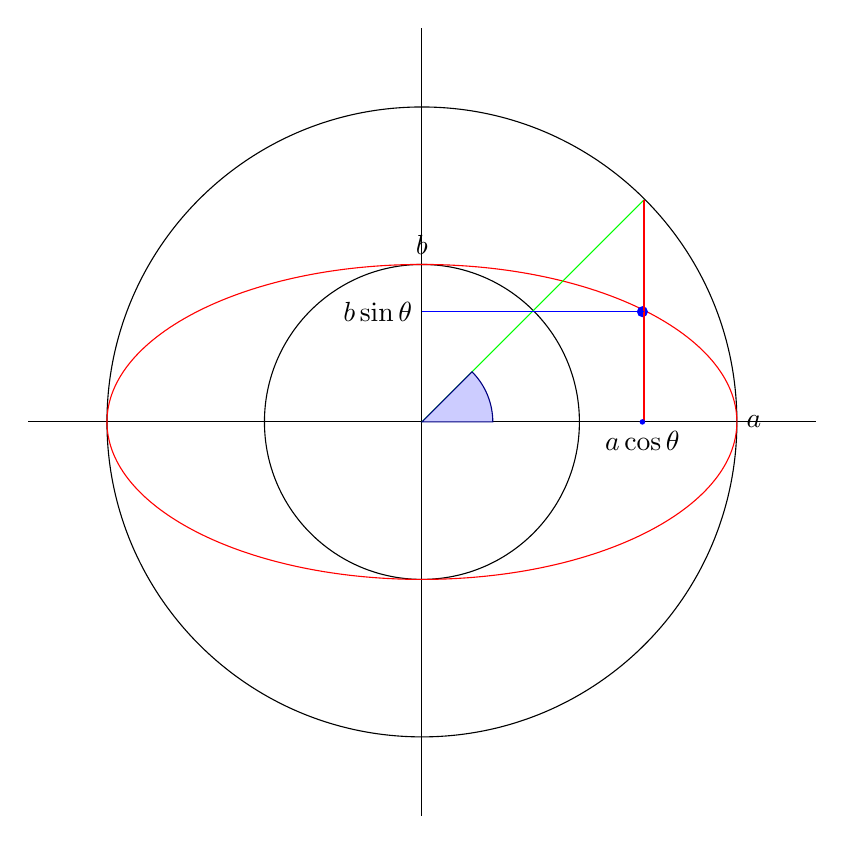
\begin{tikzpicture}
\draw (-5.0,0) -- (5.0,0); 
\draw (0,-5.0) -- (0,5.0);
\draw (4.0,0) coordinate [label= right:$a$] (a);
\draw (0,2.0) coordinate [label= above:$b$] (b);
 \draw [color=black] circle(4cm);
 \draw [color=black] circle(2cm);
\draw [color=red] (0,0) ellipse (4cm and 2cm);

\draw [color=green] (0,0) coordinate (a_1) -- (2.82,2.82) coordinate (a_2);
\fill[blue] (2.8,1.4) circle (2pt);
\draw [color=red] (2.82,2.82) coordinate (a_3) -- (2.82,0) coordinate (a_4);
\coordinate (c) at (intersection of a_1--a_2 and a_3--a_4);
%\fill[blue] (c) circle (2pt);
%\draw [color=blue] (c) -- (0,2.82) coordinate (c_2);
\draw [color=blue] (2.82,1.4) coordinate (c_3) -- (0,1.4) coordinate (c_4);

%\coordinate (d) at (intersection of a_1--a_2 and c_3--c_4);
%\fill[blue] (d) circle (2pt);
\filldraw[fill=blue!20!white, draw=blue!50!black]
(0,0) -- (9mm,0mm) arc (0:45:9mm) -- cycle;

\draw (2.8,0) coordinate [label= below:$a\cos \theta$] (acos);
\fill[blue] (acos) circle (1pt);
\draw (0,1.4) coordinate [label= left:$b\sin \theta$] (asin);
\end{tikzpicture}
\caption{}
\label{fig:ellipse1}
\end{figure}


%%% NEW 
\begin{figure}[h!tpb]
\centering
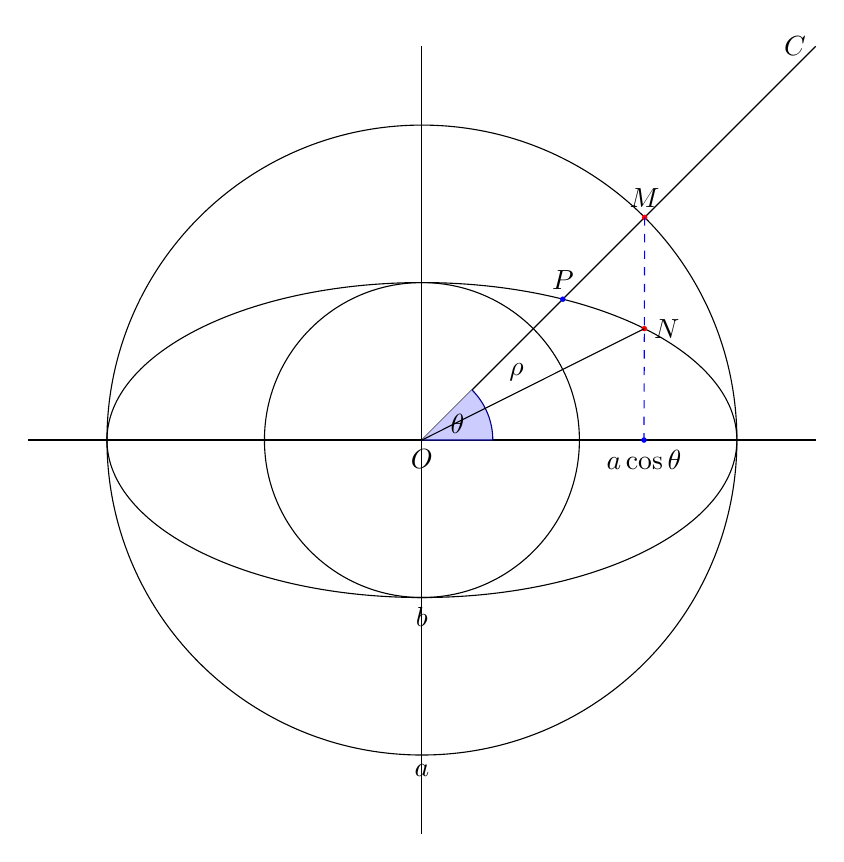
\begin{tikzpicture}
\usetikzlibrary{shapes,snakes}
\usetikzlibrary{calc,intersections,through,backgrounds}

\draw (-5.0,0) -- (5.0,0); 
\draw (0,-5.0) -- (0,5.0);

\coordinate [label=below:$O$] (A) at (0,0);
\coordinate (B) at (2.0,0.0);
\coordinate (B2) at (4.0,0.0);
\coordinate [label=left:$C$] (C) at (5,5);
\coordinate [label=below:$a \cos \theta$] (acos) at (2.82,0);
\coordinate [label=below:$\rho$] (ro) at (1.2,1.1);


\draw (A) -- (B);
\node (D) [name path=D,draw,circle through=(B),label=below:$b$] at (A) {};
\node (E) [name path=E,draw,circle through=(B2),label=below:$a$] at (A) {};
\node (F) [name path=F,draw,ellipse, minimum height=4cm,minimum width=8cm] at (A){};
\draw [name path=A--C] (A) -- (C);


% Name the coordinates, but do not draw anything:
\path [name intersections={of=F and A--C}];
\coordinate [label=above:$P$] (i-1) at (intersection-1);
\fill[blue] (i-1) circle (1pt);

\path [name intersections={of=E and A--C}];
\coordinate [label=above:$M$] (j-1) at (intersection-1);
\fill[red] (j-1) circle (1pt);

\filldraw[fill=blue!20!white, draw=blue!50!black]
(0,0) -- (9mm,0mm) arc (0:45:9mm);
\draw(25:5mm) node {$\theta$};

\draw [name path=M--acos,dashed,blue] (j-1) -- (acos);
\fill[blue] (acos) circle (1pt);

\path [name intersections={of=M--acos and F}];
\coordinate [label=right:$N$] (k-1) at (intersection-1);
\fill[red] (k-1) circle (1pt);

\draw [name path=A--N] (A) -- (k-1);










\end{tikzpicture}
\caption{}
\label{fig:ellipse1}
\end{figure}





, and the radii of the two circles are the lengths of the
semi-minor and semi-major axes.



\begin{thebibliography}{0}
\bibitem{ja} M. Barranco and J. R. Buchler, {\it Phys. Rev.}
{\bf C34}, 1729 (1980).

\bibitem{ballard} D. H. Ballard, Generalizing the Hough Transform to
  detect Arbitrary Shapes. (1979).

\bibitem{nixon} M. Nixon and A. Aguado. Feature Extraction and Image
  Processing.

\end{thebibliography}

\end{document}
